%\documentclass[10pt,conference]{IEEEtran}
% If the IEEEtran.cls has not been installed into the LaTeX system files,
% manually specify the path to it:
\documentclass[conference]{/home/pranav/Desktop/Publication_work/latex_class_files/IEEEtran}
\usepackage[]{amsmath}
\usepackage[pdftex]{graphicx}
\usepackage{url}
\usepackage{subfig}
\usepackage{tabularx}


\begin{document}

% paper title
\title{Achieving seamlessness in Multiprojector displays using camera feedback}


% author names and affiliations
% use a multiple column layout for up to three different
% affiliations



\author{
    \IEEEauthorblockN{Pranav Kant Gaur\IEEEauthorrefmark{1}, Dinesh M. Sarode\IEEEauthorrefmark{1}, S.K. Bose\IEEEauthorrefmark{1}}
    \IEEEauthorblockA{\IEEEauthorrefmark{1}Computer Division, Bhabha Atomic Research Centre
    \\\{pranav,dinesh,bose\}@barc.gov.in}
}
    



\maketitle

\begin{abstract}
High resolution displays utilizing an array of commodity projectors(popularly called \textit{Tiled displays}) are becoming popular approach for visualizing high resolution content like scientific datasets[1]. These systems provide a relatively cheaper and flexible alternative to displays based on single high resolution monitor or projector. This approach inherently provides a method to create displays with resolution much higher than that possible by using a single high resolution display device. In this paper, we describe algorithms for geometric alignment of projection regions of grid of arbitrarily placed projectors and attenuation of projected intensities in the overlapping regions of multiple projectors. Combination of these algorithms help us achieve a seamless high resolution display. We also propose a novel technique based on \textit{cross ratio} invariant for utilizing full projection region of individual projectors which was limited by the size of features used for geometric alignment in the earlier approach[2]. This also results in more imperceptible edge blending artifacts for same physical setup of projectors.
\end{abstract}


\section{Introduction}
Tiled displays provide an alternative to the visualization of high resolution content over single large scale high resolution monitor(or projector) by attaining comparable performance using combination of low cost and low resolution commodity displays. Tiled displays have been realized either using grid of monitors[3-5] or projectors[2][6-8]. Using LCD monitors provides a compact, relatively cheaper and readily configurable high resolution visualization solution, though it still cannot completely imitate a single high resolution display because bezels of monitors obstruct the geometric continuity of the rendered content. Further, they are not easily portable because of rigid arrangement of monitor panel grid. Whereas in a multiprojector system, projectors may be arbitrarily placed and they inherently do not enforce any limitations of physical seams. In our work, we have opted to utilize projectors to achieve \textit{seamless} rendering of content. \par
Projectors will project quads without necessarily ensuring geometric continuity over the projected content. Manual \textit{keystoning} to geometrically align content from multiple projectors on the screen is time consuming and tedious. Further, it can easily become impractical for large number of projectors. To automate geometric alignment we have used camera as a feedback device for projectors. Our earlier attempted approach was based on the concept of \textit{Homography}\cite{9}. It establishes planar projective mapping between screen and camera followed by that between camera and projector. Utilizing combination of these homographies it computes relation between screen and projector. It is assumed that position of final projection on the screen is known, therefore corresponding projector space coordinates can be easily computed utilizing screen to projector homography. Using this information output from all projectors are mapped to well defined identical rectangular regions on the screen. Collectively, this results in a seamless projected content on the screen. Screen and projector coordinates are related via camera coordinate system as,\newline
Homography between points on screen($x_s$) and camera($x_c$), $H_{sc}$
\begin{equation}
x_{c}=H_{sc}*x_{s}
\label{hsc}
\end{equation}
Similarly, homography between points on camera($x_c$) and projector($x_p$), $H_{cp}$
\begin{equation}
x_{p}=H_{cp}*x_{c}
\label{hcp}
\end{equation}

Therefore, using screen-projector homography, $H_{sp}$ gives,
\begin{equation}
x_{p}=\underbrace{H_{sc}*H_{cp}}_{H_{sp}}*x_{s}
\end{equation}

However, this approach assumes accurate positioning of features on the screen. Further, pre-positioning of projection region results in relatively stringent physical constraints on placement of projectors.\par

Brown's[2] approach relaxes that assumption and instead allows for a casual positioning of projectors. It aims to create geometrically seamless and rectangular image in camera space which guarantees geometrical seamlessness on the screen. But it does not guarantee rectangular output on the screen. Further, the usable projection region is limited by the size of features used for geometric registration.  

However, Brown's approach has an advantage of being much more flexible in terms of projector placement, hence we selected it as our base approach on top of which we have removed its limitations mentioned above.\par

Since neighboring projectors may have overlap in their projection regions resulting in brighter regions at their boundaries, it is necessary to attenuate the intensity of projected images in such regions so that overall projected content appears \textit{seamless}. This problem is called \textit{edge blending}.

\section{Geometric alignment}
In our work, we have used an approach similar to that proposed in [2] but with some enhancements. Specifically, geometric alignment in [2] limits the usable projection region of each projector to the region within the quad of outermost features used for geometric alignment. In this work, we have proposed to utilize \textit{cross ratio} invariance which is preserved between perspective projection from projector to planar screen and planar screen to camera in order to recover entire projection region of individual projectors. This increases the overall projection region as shown in figures \ref{non_cross_rat} and \ref{cross_rat}. It also eliminates another implicit limitation of [2] which requires neighboring projectors to overlap atleast upto their outermost features to ensure geometric continuity, which limits the flexibility of positioning of individual projectors. 


\subsection{Cross ratio invariance}
Cross ratio is a planer projective invariant. It states that: Given 4 collinear points A,B,C,D,(arranged geometrically in the same order) their cross-ratio $CR$:
\begin{equation} 
CR[A,B,C,D]=\frac{\frac{AC}{AD}}{\frac{BC}{BD}}
\label{cross_rat}
\end{equation}
will be preserved under perspective projection. Therefore, assuming planer perspective projection of features from projector to screen and from screen to camera, we can recover coordinates of an unknown point(say 'A') in camera space given coordinates of other three(i.e.,'B','C','D' are known). \newline \newline
Let $A_p$,$B_p$,$C_p$,$D_p$ be the coordinates of 4 collinear points in projector space and $A_c$,$B_c$,$C_c$,$D_c$ be the corresponding projection in camera space. Here, $B_c$,$C_c$ and $D_c$ are known whereas $A_c$ is unknown but $A_p$,$B_p$,$C_p$,$D_p$ are all known. Let us further represent the line joining $A_c$,$B_c$,$C_c$,$D_c$ in parametric form as:
\begin{equation}
\begin{aligned}
x_t=B_c^x+t*(D_c^x-B_c^x)\\
y_t=B_c^y+t*(D_c^y-B_c^y)
\end{aligned}
\label{paramet}
\end{equation}
where, $(x_t,y_t)$ are parametric coordinates of an unknown point(in our case $A_c$)\newline
Utilizing cross ratio invariance yields following relation:
\begin{equation}
CR_p=\frac{|AC|_c*|BD|_c}{|BC|_c*|AD|_c}
\label{cross_rat_eqn}
\end{equation}
Here $CR_p$ is the cross ratio computed in projector-space, $|ab|_c$ represents euclidean distance between points $a$ and $b$ in camera-space. Using equation 5, we get quadratic equation with following possible solutions:
\begin{equation}
\begin{aligned}
t_1=\frac{-b+\sqrt{b^{2}-4ac}}{2a}\\
t_2=\frac{-b-\sqrt{b^{2}-4ac}}{2a}
\end{aligned}
\label{quad_eqn}
\end{equation}
where,\newline
Let,\newline
$delta={CR_p*(\frac{|BC|_c}{|BD|_c})}^2$\newline
Then,
\newline
$a=(1-delta)*|BD|_c^2$\newline
\begin{eqnarray*}
b=2*{(D_c^x-B_c^x)*(B_c^x-C_c^x)+(D_c^y-B_c^y)*(B_c^y-C_c^y)} \\ + 2*|BD|_c^{2}*delta
\end{eqnarray*}
$c=|BC|_c^2-delta*|BD|_c^2$ \newline


Based on the convention of the chosen coordinate system, only one of $t_1$ or $t_2$ will be the valid position of the unknown point $A_c$. Figure \ref{cross_rat_img} shows application of this concept on a camera image where an unknown point $A_c$(shown using \textit{red} solid circle) can be recovered using known \textit{collinear} points $B_c$,$C_c$,$D_c$(all shown using \textit{white} solid circles) . Details on how this approach has been used to recover full projection region are given in \textit{Algorithms} subsection.

\begin{figure}
\centering
\def\tabularxcolumn#1{m{#1}}
\begin{tabularx}{\linewidth}{@{}cXX@{}}
\begin{tabular}{c c}
\subfloat[]{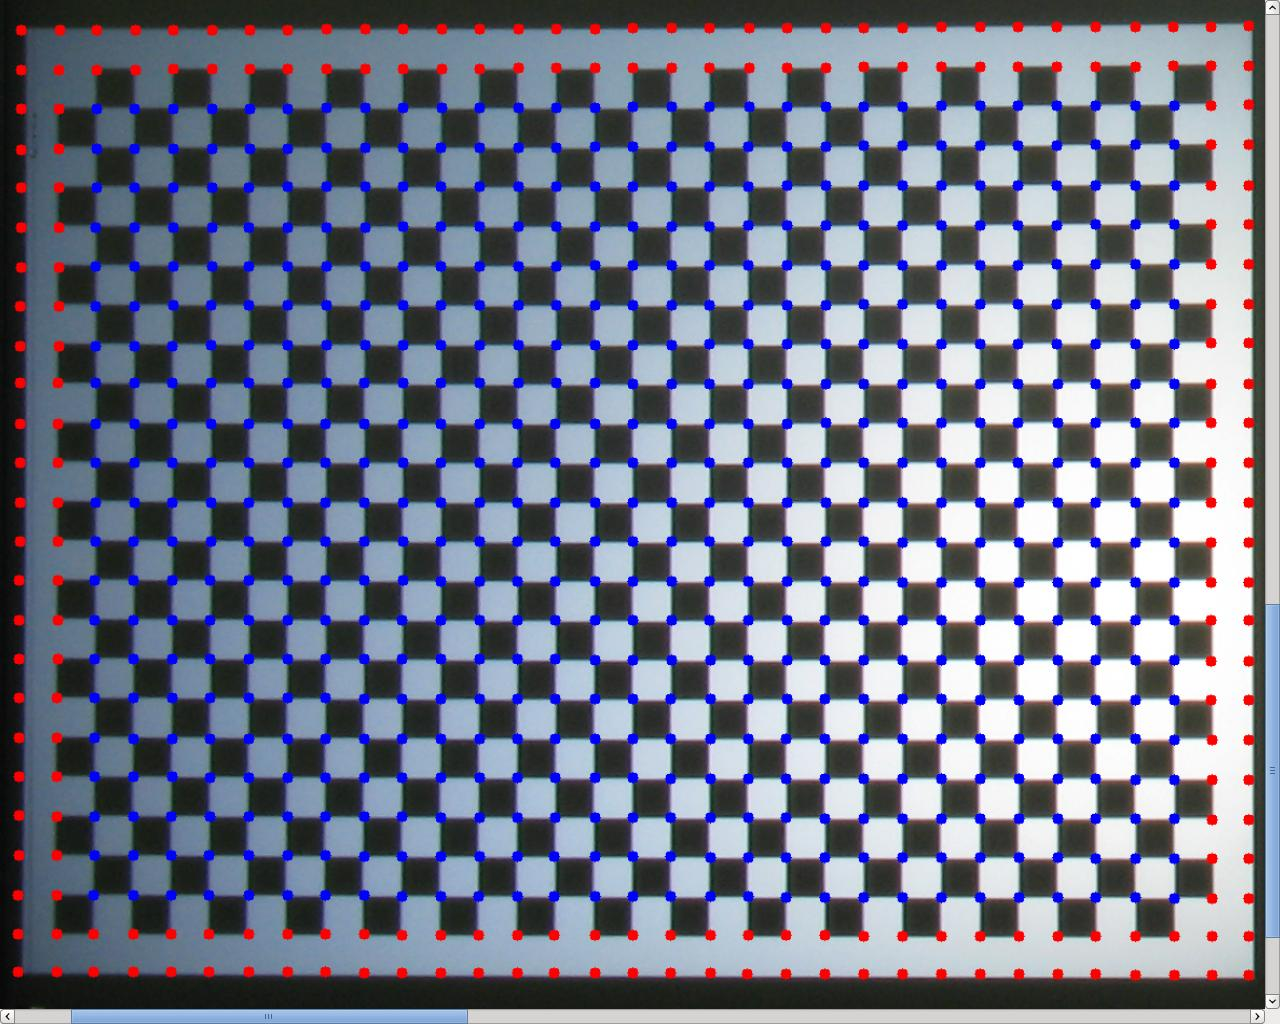
\includegraphics[width=4cm,height=4cm]{figures/cross_ratio_points.jpg}} & 
\subfloat[]{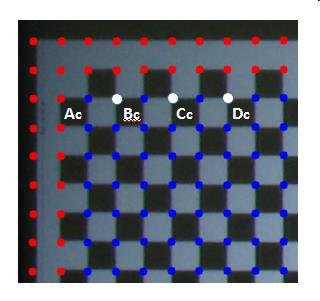
\includegraphics[width=4cm,height=4cm]{figures/cross_ratio_find_point.jpg}} \\
\end{tabular}
\end{tabularx}
\caption{Recovering $A_c$ using $B_c$,$C_c$,$D_c$}
\label{cross_rat_img}
\end{figure}

\subsection{A note on Chromium}
Chromium[10] is a framework for enabling single desktop OpenGL based graphics application to be transparently portable to distributed display composed of an arrangement of multiple display elements like monitors, projectors. It accomplishes this by intercepting the OpenGL calls initiated by applications and distributing them to individual displays according to logical layout(called \textit{chromium tile configuration}) of the multi-element(monitor or projector) display. This process is transparent to the application, resulting in no additional overhead on part of application developer to add support for multiple displays. \par
In our work, we have used chromium framework to utilize multiprojector display for conventional unmodified OpenGL applications. Specifically, we modify the \textit{chromium tile configuration} and \textit{texture mapping} information for achieving multiprojector geometric alignment which is transparent to the applications. In order to achieve seamlessness, \textit{alpha maps} are generated for each projector which are used for attenuating the image intensity in the overlap region.

\subsection{Algorithms}
In order to achieve geometric alignment of the content projected by multiprojector setup we calculate the rectangular share of each projector in the global image to be projected in the form of \textit{tile configuration}. Once the image is partitioned, texture mapping information is computed for each projector to map its share to the correct location in its vertex space. This mapping is also called \textit{warping}. Complete process of geometric alignment is partitioned into two major steps:\textit{feature detection and regularization} and \textit{warp map computation}.   
\begin{enumerate}    
\item Feature detection and regularization:
\begin{enumerate}
\item Projector projects checkerboard features.
\item Camera captures features.
\item Since collinearity is invariant under projective transformation, features collinear in projector image must be 		      collinear in camera space also. In order to account for this, detected locations of features in camera image are regularized by explicitly enforcing collinearity constraint. Specifically, each feature is computed as intersection of vertical and horizontal fitted lines.

\item Once the features are regularized, lost projection region at the boundary are recovered using Cross-ratio constraint(using equation \ref{quad_eqn}).
\item Regularized positions of newly computed coordinates(in step (d)) are computed by fitting line on collinear points and computing intersections.\newline
\end{enumerate}
\item Warping map computation:
\begin{enumerate}	     
\item Local bounding boxes are computed for each projection region in camera space. These boxes are the convex hulls enclosing all features of a projector recovered in feature detection and regularization phase.

\item A global bounding box is computed which is convex hull enclosing all local bounding boxes.

\item This global bounding box acts like a global coordinate system containing all local bounding boxes and hence all the 		      detected features. 
\item  A \textit{maximal} box is computed which can contain any local bounding box. Naturally, it corresponds to the box having maximum width and height among that of all local bounding boxes. Scales along X and Y axes are computed using maximum width and height. All local bounding boxes are modified to have maximum width and height.
 
\item These width and height are equated with buffer width and height of individual projectors to maintain uniform pixel size regardless of different sizes of projection region for different projectors on the screen. This defines the global tile configuration for given multiprojector setup.

\item To compute texture coordinates corresponding to all features in a projector space, normalized coordinates of all features are 	            computed with respect to its local bounding box origin.
\end{enumerate}
\end{enumerate}
Algorithm computes Chromium tile configuration and Vertex-texture mapping for each projector. For visual description of warping map computation process reader is referred to [2].

\section{Edge blending}
Edge blending algorithm attempts to attenuate the intensity of projected images from overlapping projectors in the common region so that seams between neighboring projectors become imperceptible. It utilizes the overlapping information acquired during geometric alignment phase for calculating attenuation(or \textit{alpha}) maps.
\subsection{Algorithm}
\begin{enumerate}
\item Transform detected coordinates to global frame in chromium coordinates system.
\item Compute polygons bounding the detected corners for each projector.
\item Scan chromium image space and for each pixel, check which projector(s) share it.
\item For every sharing projector, assign that pixel the id of that projector.
\item Compute alpha weight of each projector based on distance transform value at that pixel for each projector.
\end{enumerate}
Algorithm computes alpha map for each projector which is a 2D array(with same dimensions as of projector image) with value corresponding to each pixel varying from 0 to 255. Alpha weight at any pixel represents its \textit{transparency}.

\section{Practical implementation}
In this section, we describe software architecture of multiprojector display system and hardware setup used for our experiments.

\subsection{Software architecture}
Software system is composed of geometric alignment module and edge blending module. Geometric alignment module computes vertex-texture map and chromium tile configuration for each projector. Edge blending module computes the alpha weights for each projector based on region of overlap among neighboring projectors. These information are sent to Master machine which runs chromium service to appropriately distribute alpha maps and vertex-texture mapping to individual slave machines driving the projectors.

\subsection{Hardware setup}
Projectors are connected through slave machines(Workstations). Single slave drives 3 projectors(a row of display grid in our case). So, there are 3 slave workstations for 3X3 grid of projectors. Each slave runs chromium service to receive and accordingly texture map images to be projected by individual projectors under its control. Warping map, chromium tile configuration and blend map are generated on remote machine connected to the cluster(master+slave arrangement) through local network connection over Ethernet. Figure \ref{setup} shows our display screen with workstation cluster and a camera which is used as a visual feedback device. Figure \ref{projs} shows the 3X3 projector grid in our rear projection display system.
\begin{figure}
\centering
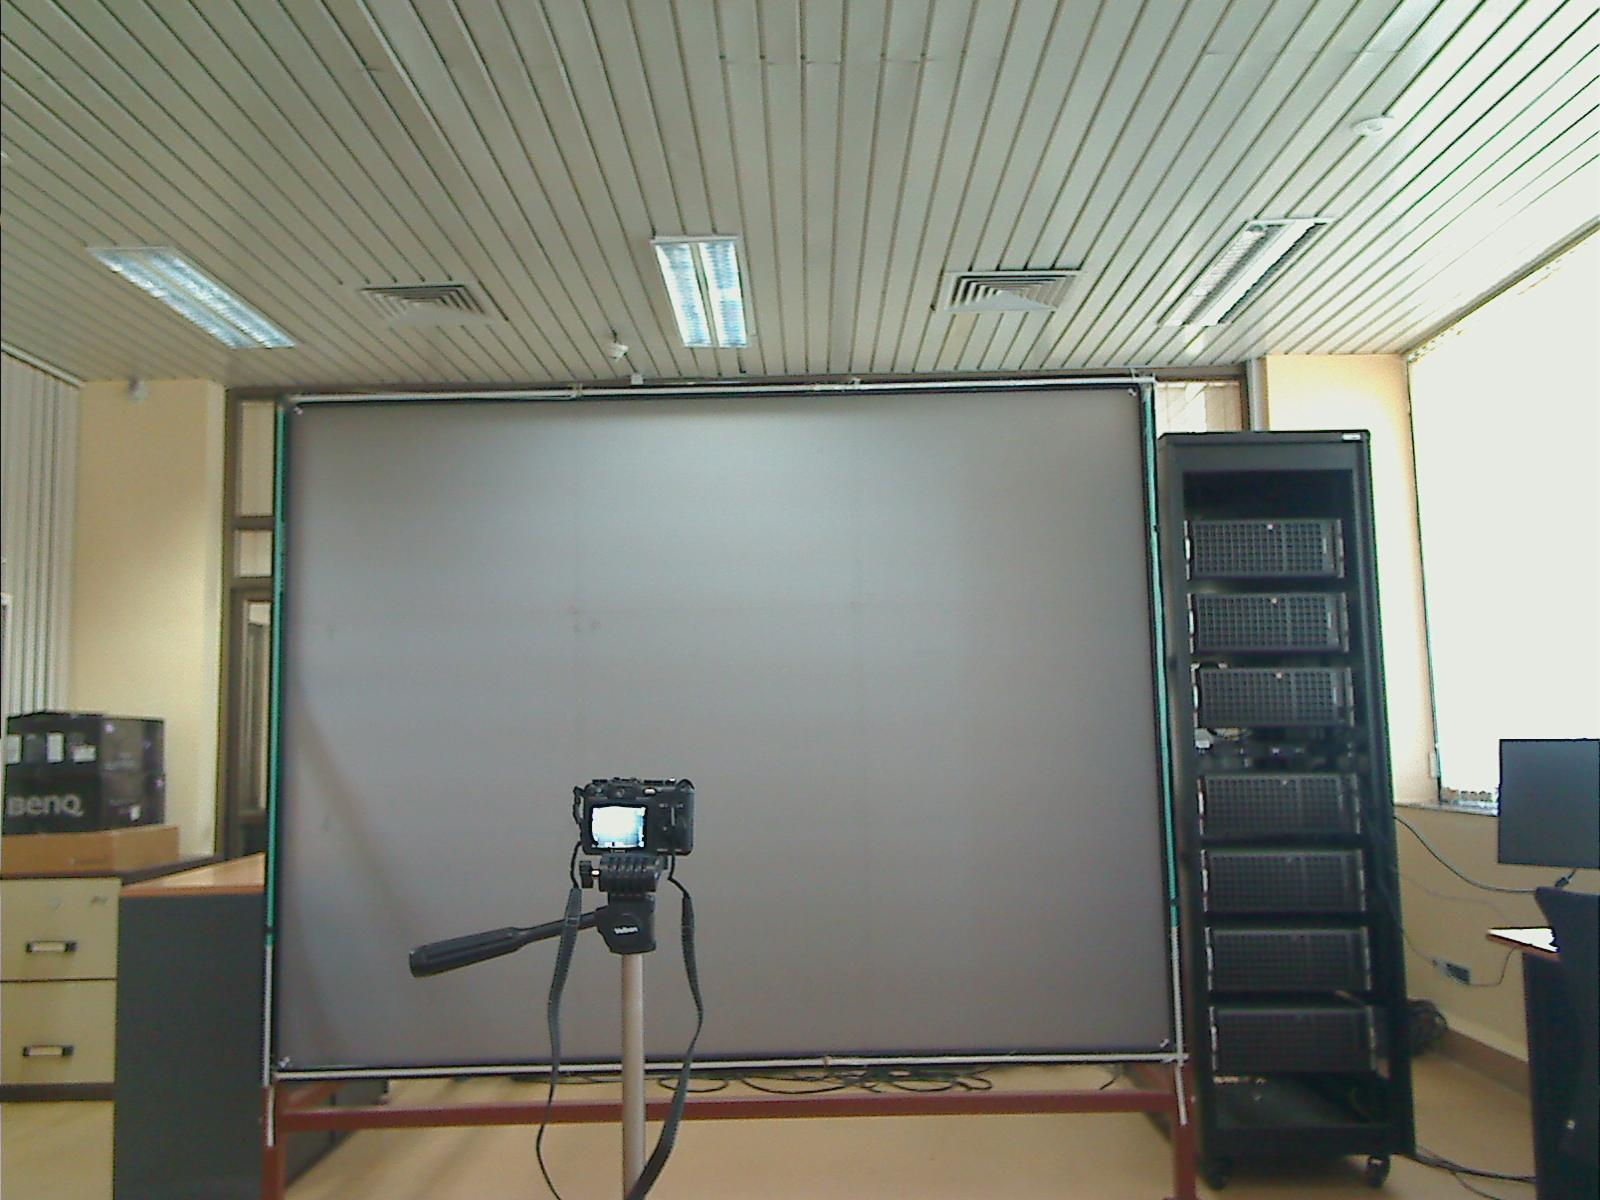
\includegraphics[width=6cm,height=4cm]{figures/setup.jpg}
\caption{System setup}
\label{setup}
\end{figure}

\begin{figure}
\centering
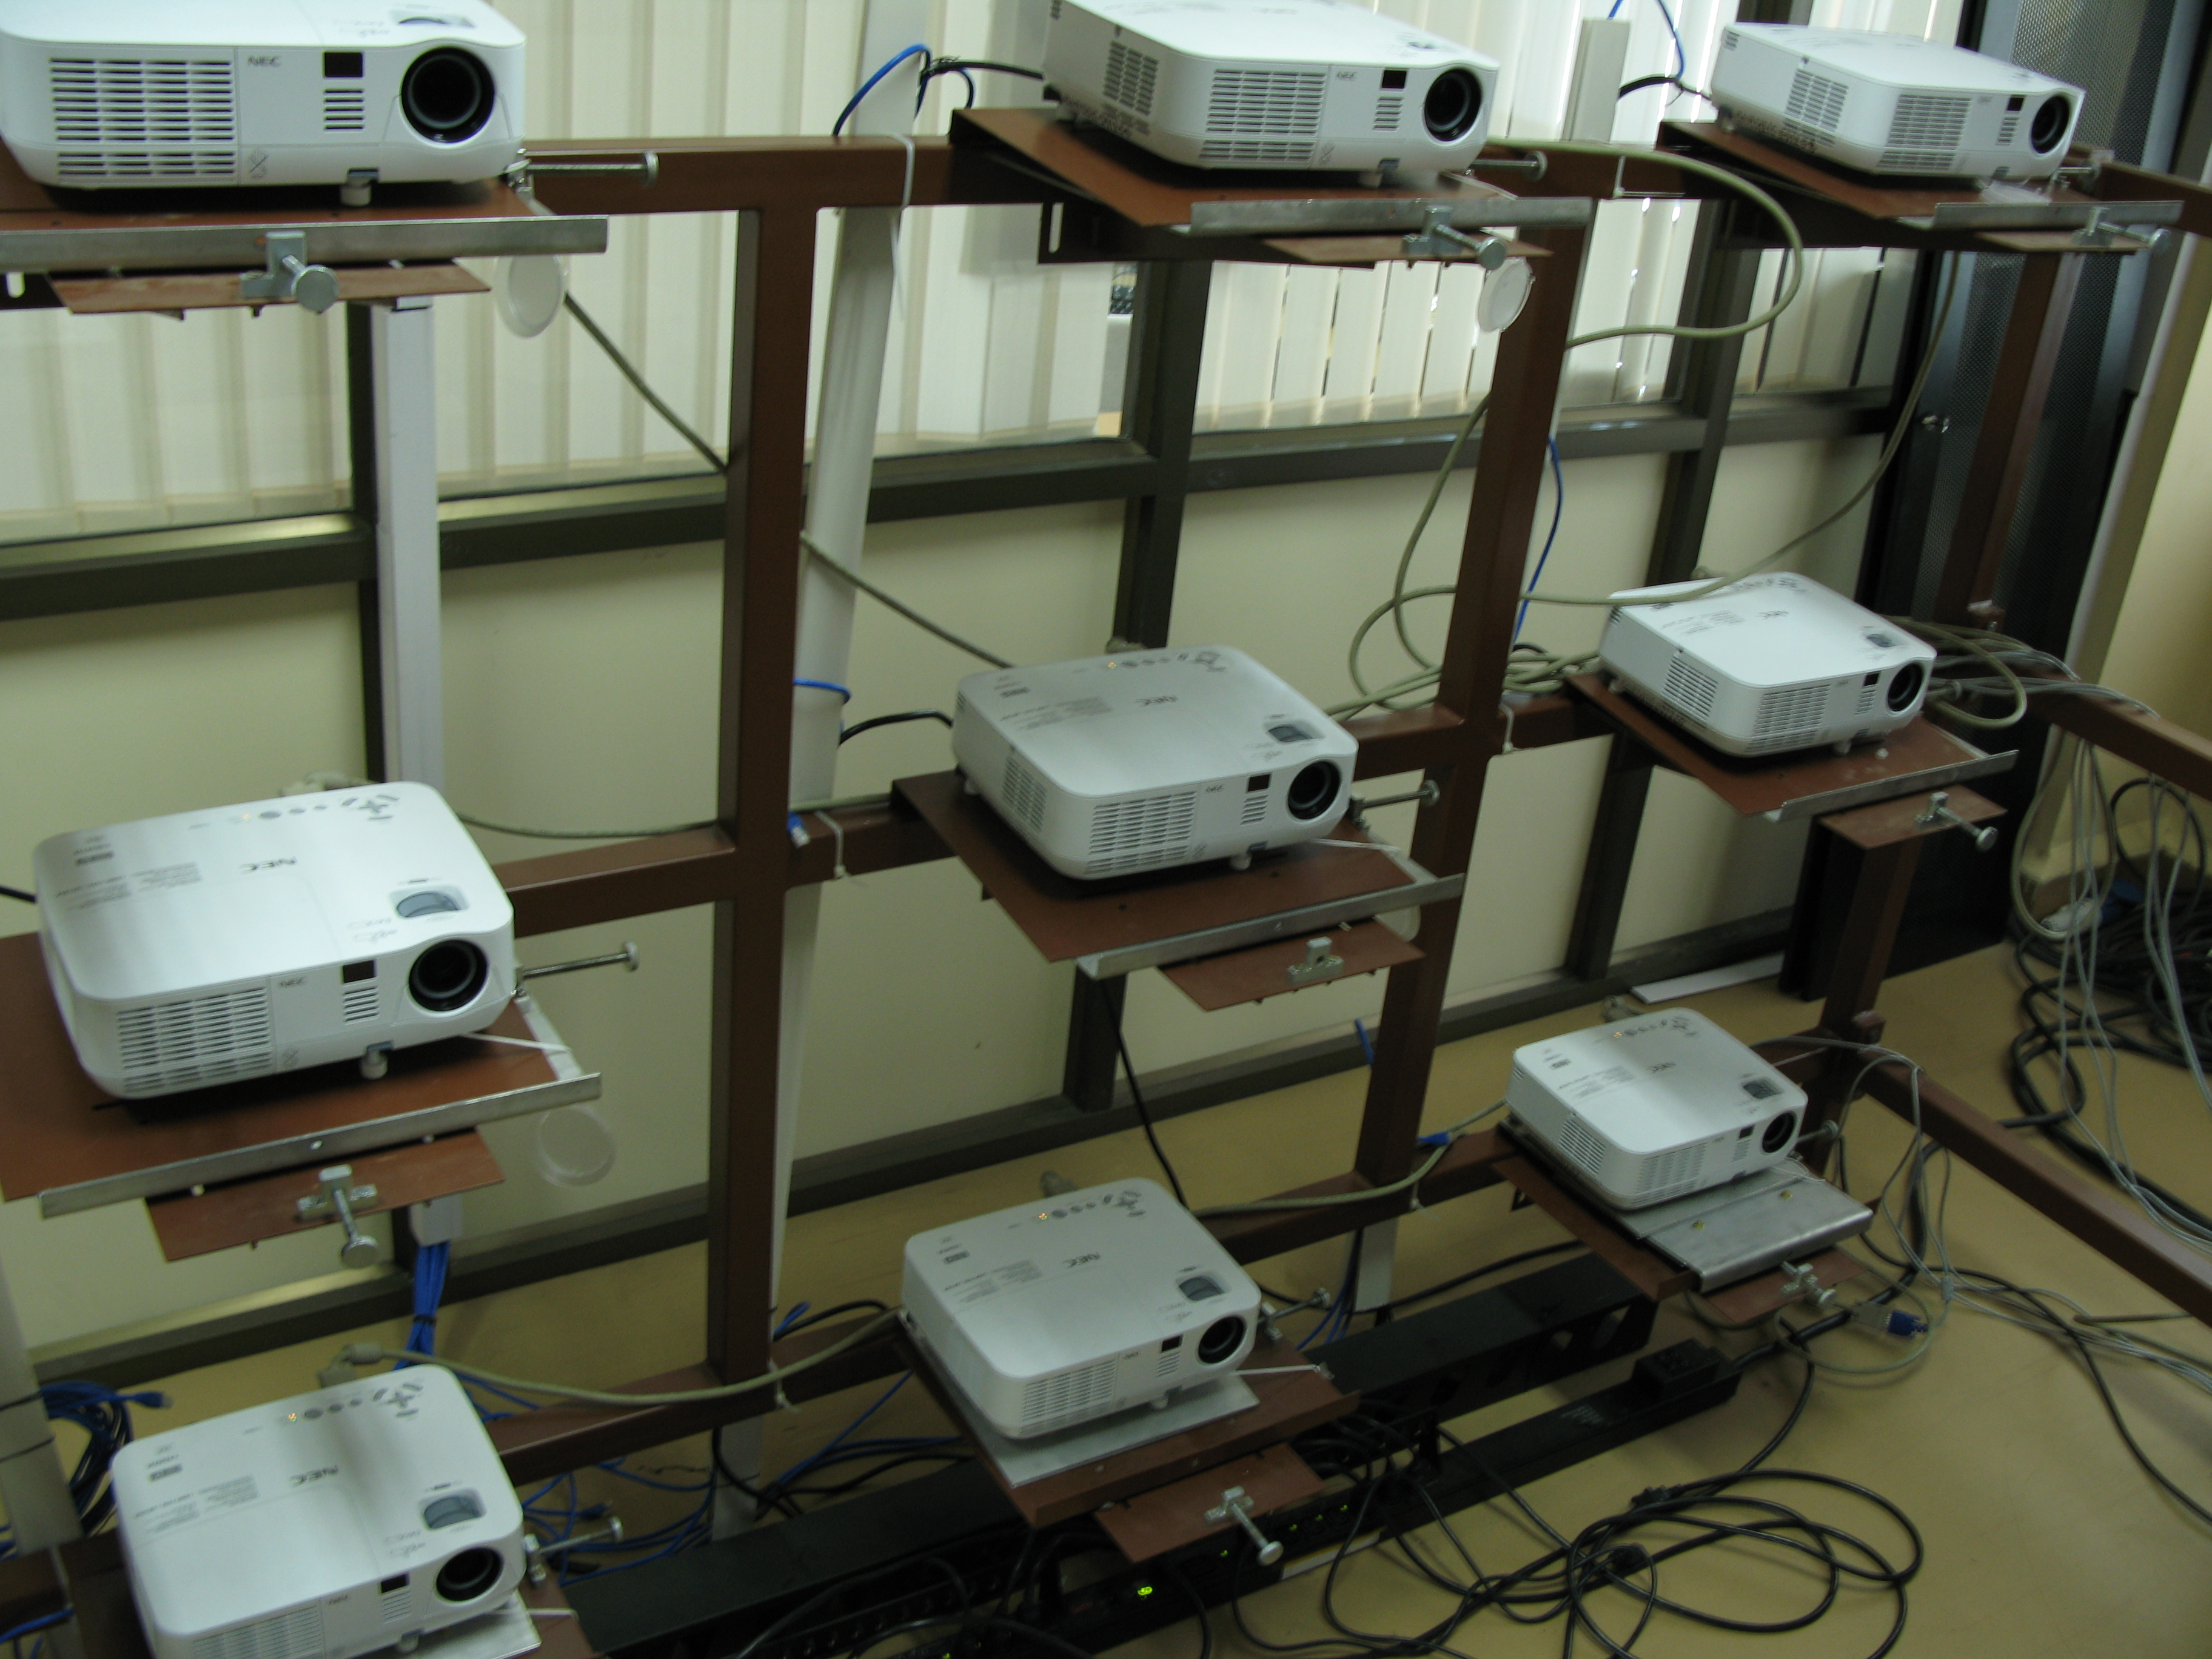
\includegraphics[width=6cm,height=4cm]{figures/projs.jpg}
\caption{3X3 rear projection grid behind the screen}
\label{projs}
\end{figure}

\subsection{Software dependencies}
OpenCV version 2.4 is used for camera image processing specifically, corner detection, image undistortion and camera calibration. GPhoto2(version 2.5.2) library is used for interfacing digital camera. Chromium(version 1.9) was modified to provide geometric correction and edge blending capability. Indigenously developed Control panel(version 1.0.2) software was used for logging into slave machines from master workstation.


\section{Results}
Figure \ref{non_cross_rat} shows the projection region without cross ratio and figure \ref{cross_rat} shows final output utilizing cross ratio constraint. Both renderings are on same physical arrangement of projectors. Full projection region was utilized in cross ratio approach(refer fig. \ref{cross_rat}) whereas projection region in approach by Brown\cite{2} was limited by feature size as shown in figure \ref{non_cross_rat}. \newline 
Further, it can be inferred that in same physical arrangement of projectors, the cross ratio based approach allows for more inter-projector overlap leading to more realistic alpha maps as can be compared in figures \ref{non_cross_rat} and \ref{cross_rat}. Consequently, boundaries are more visible in figure \ref{non_cross_rat} as compared to those in figure \ref{cross_rat}.

\begin{figure}
\centering
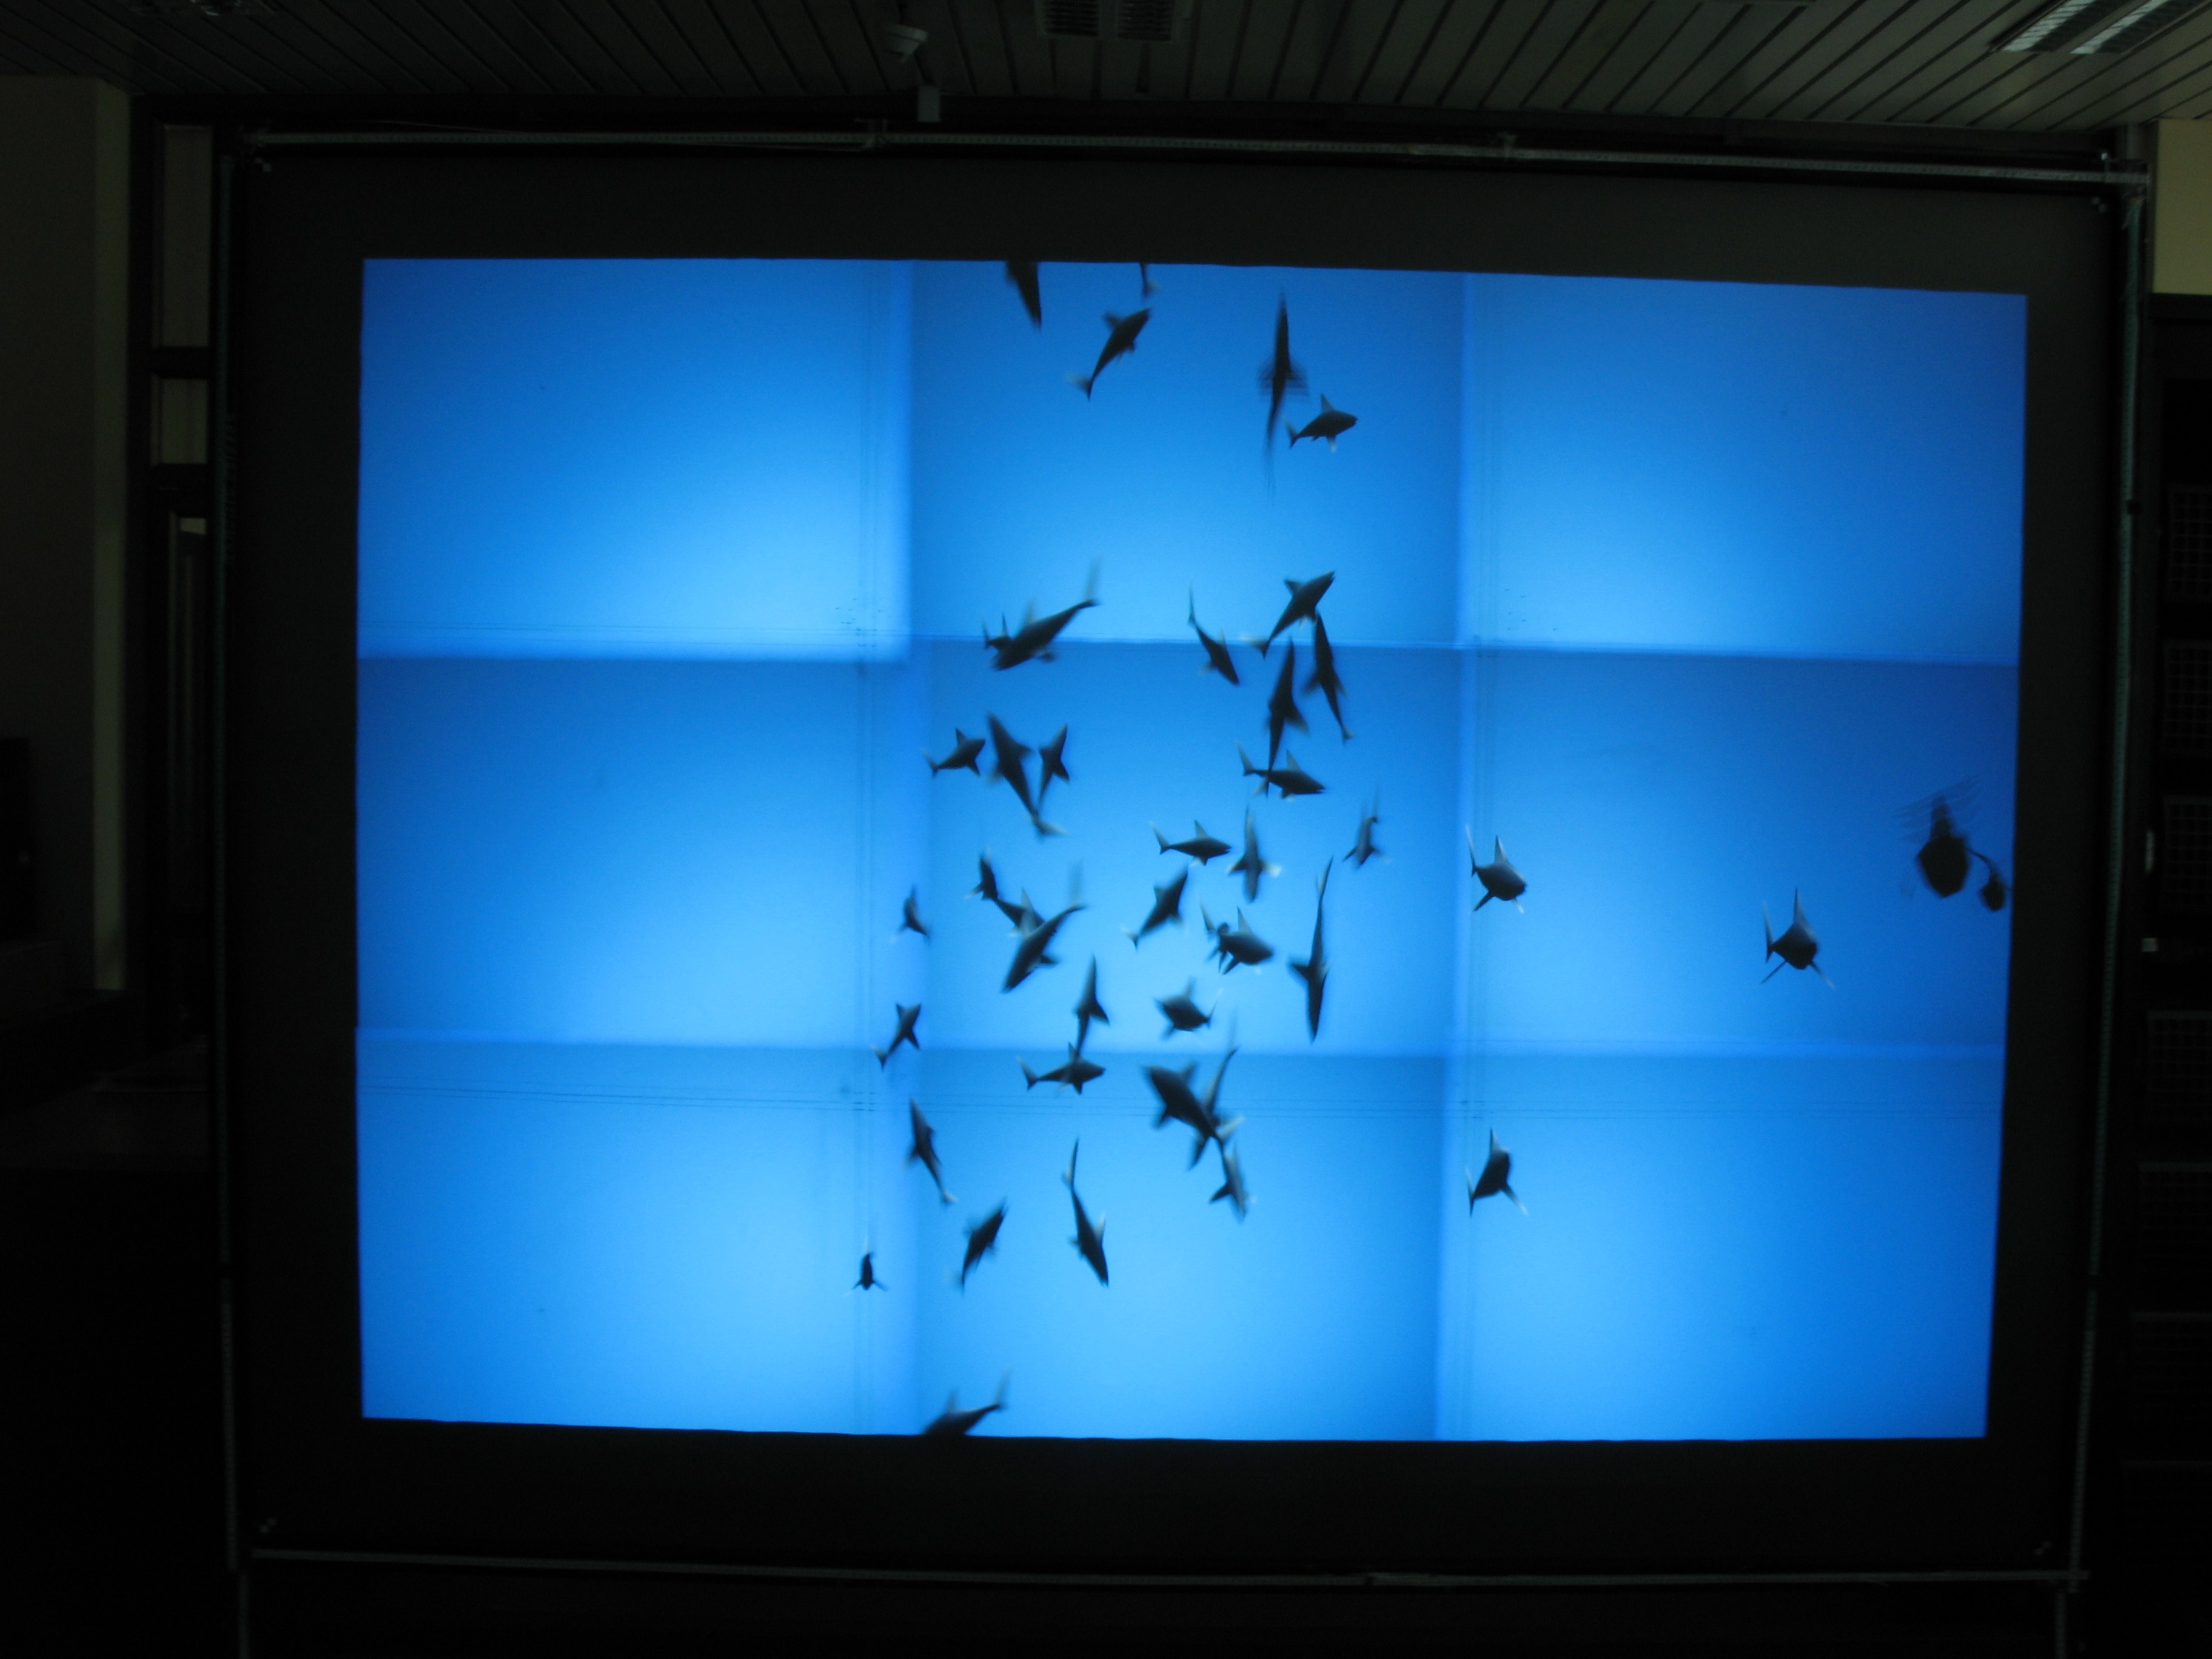
\includegraphics[width=6cm,height=4cm]{figures/without_cross_rat.jpg}
\caption{Without cross ratio}
\label{non_cross_rat}
\end{figure}


\begin{figure}
\centering
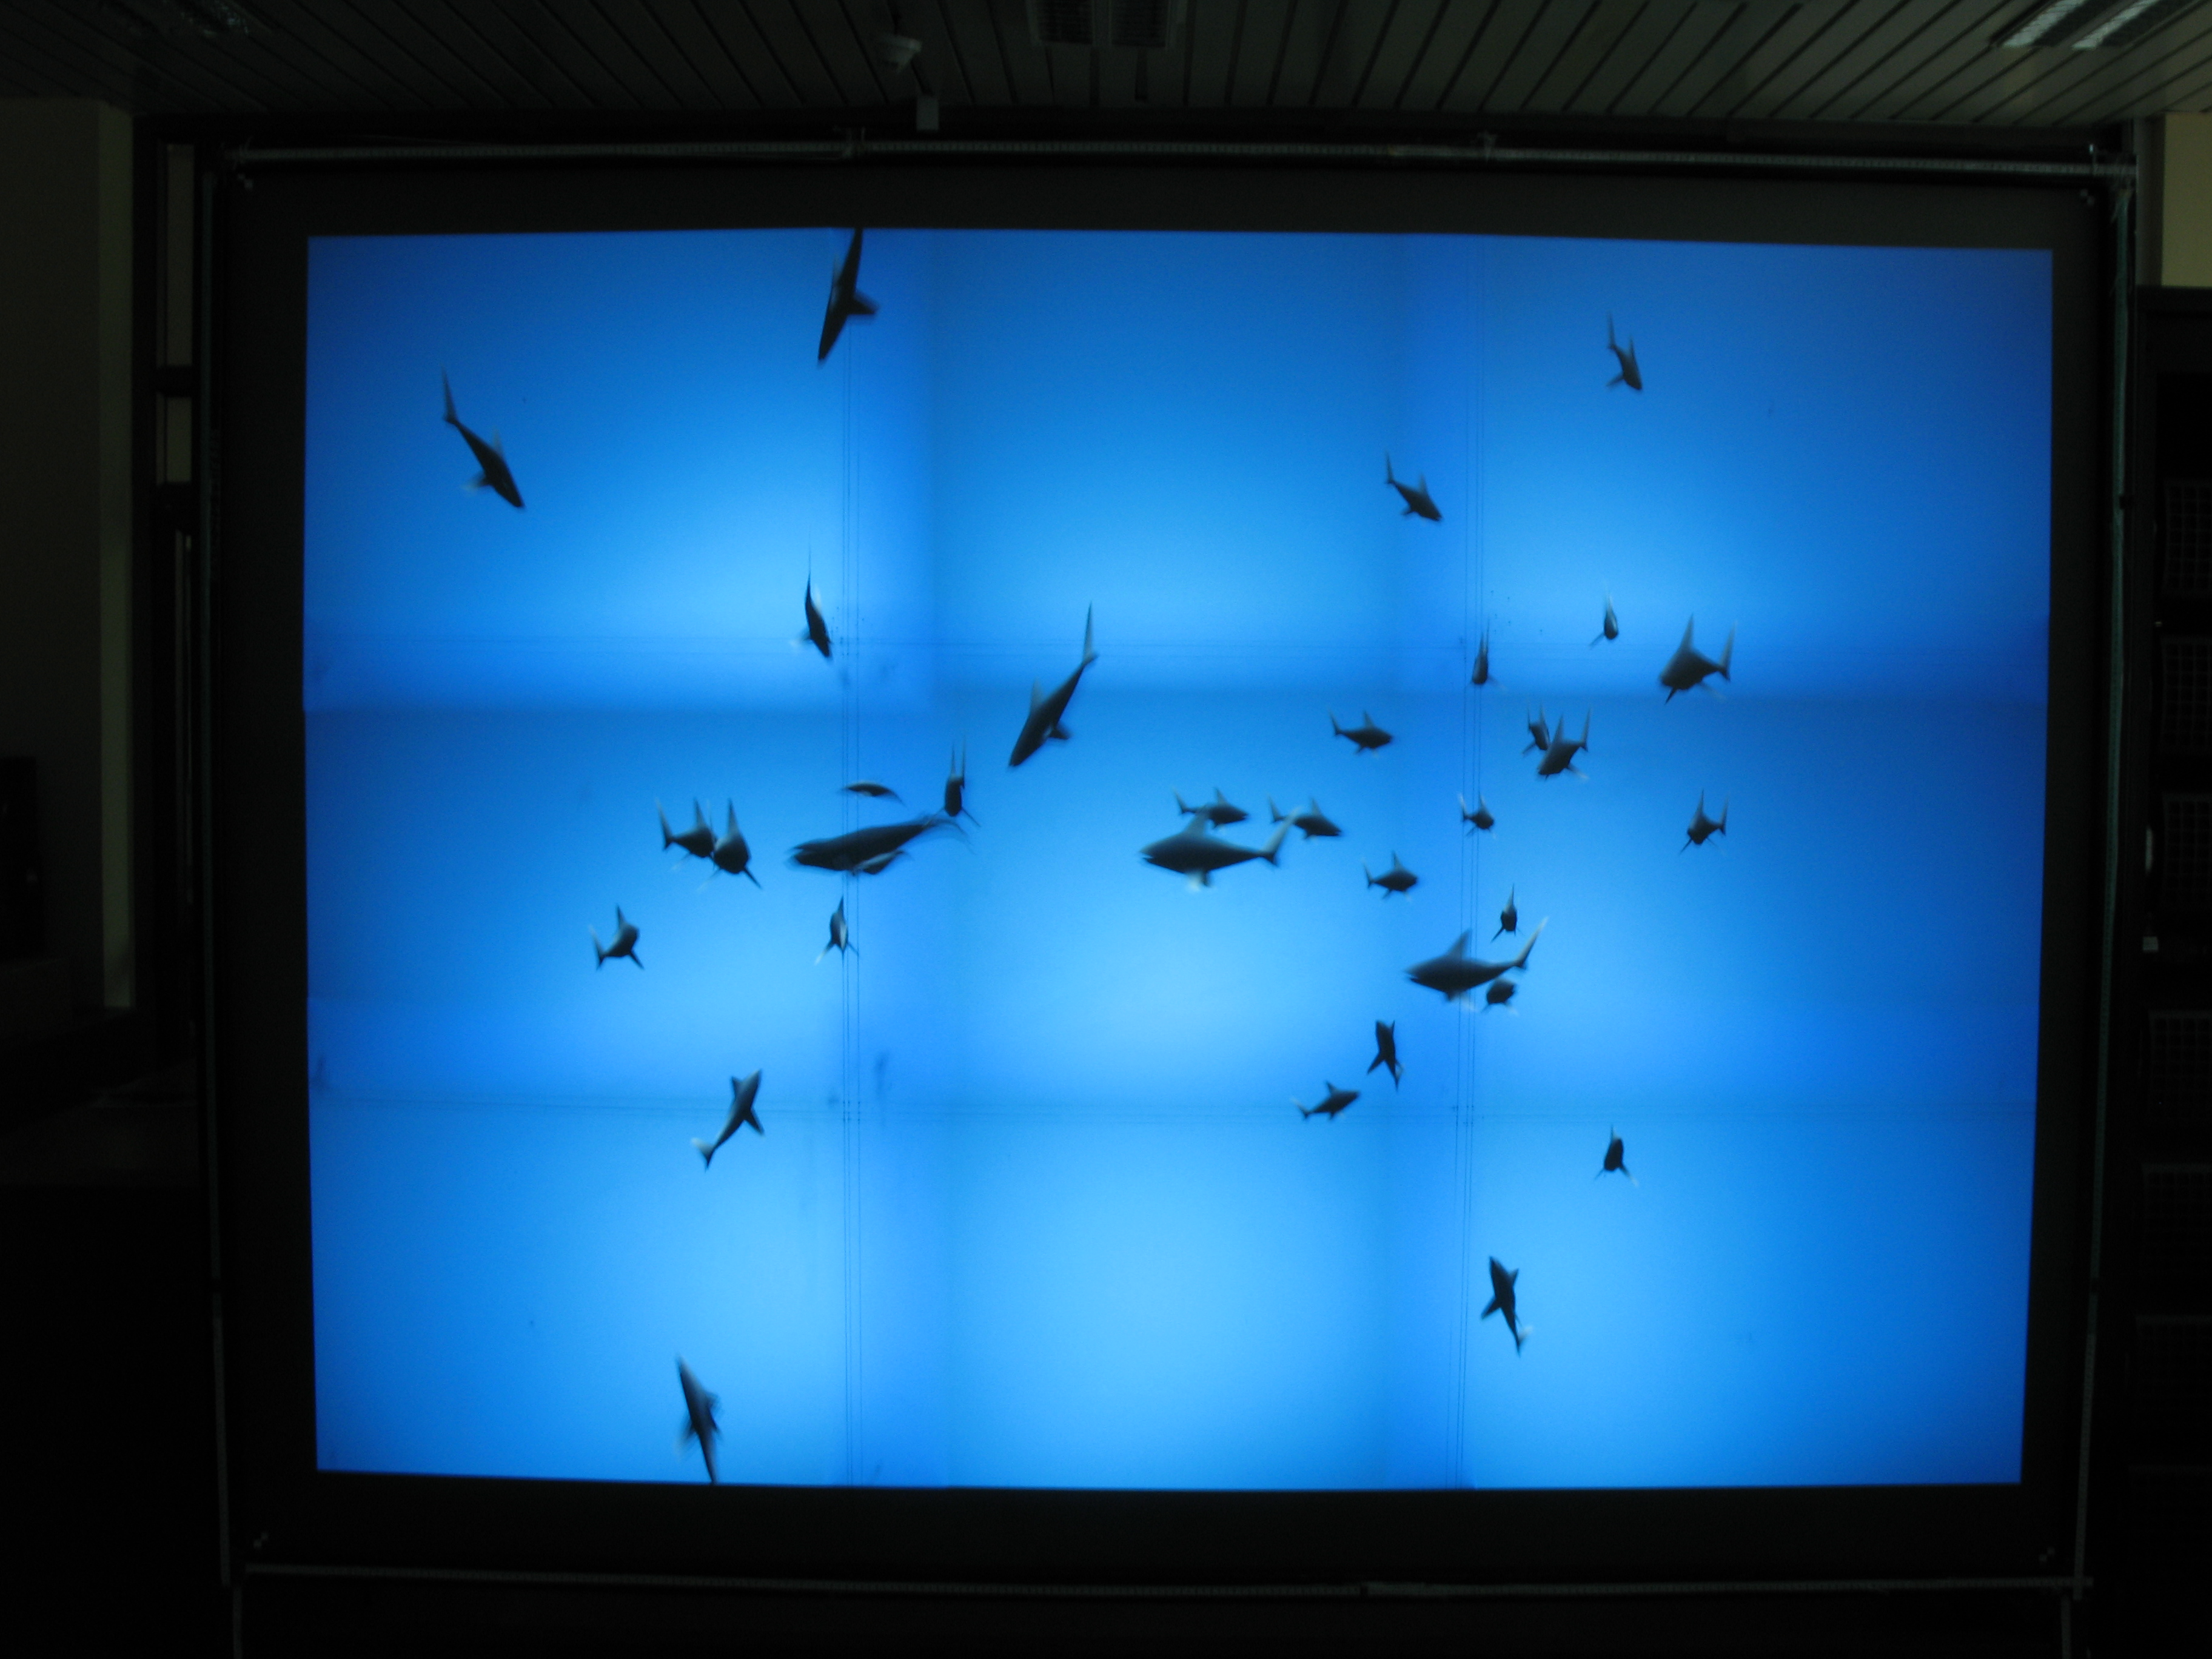
\includegraphics[width=6cm,height=4cm]{figures/with_cross_rat.jpg}
\caption{With cross ratio}
\label{cross_rat}
\end{figure}

\subsubsection{Geometric alignment accuracy}
Maximum misalignment on screen was found to be about 2.5mm across all inter-projector boundaries. A grid was projected across the display, figure \ref{misalign} shows the magnified view of maximum inter-projector misalignment observed after geometric registration.

\begin{figure}
\centering
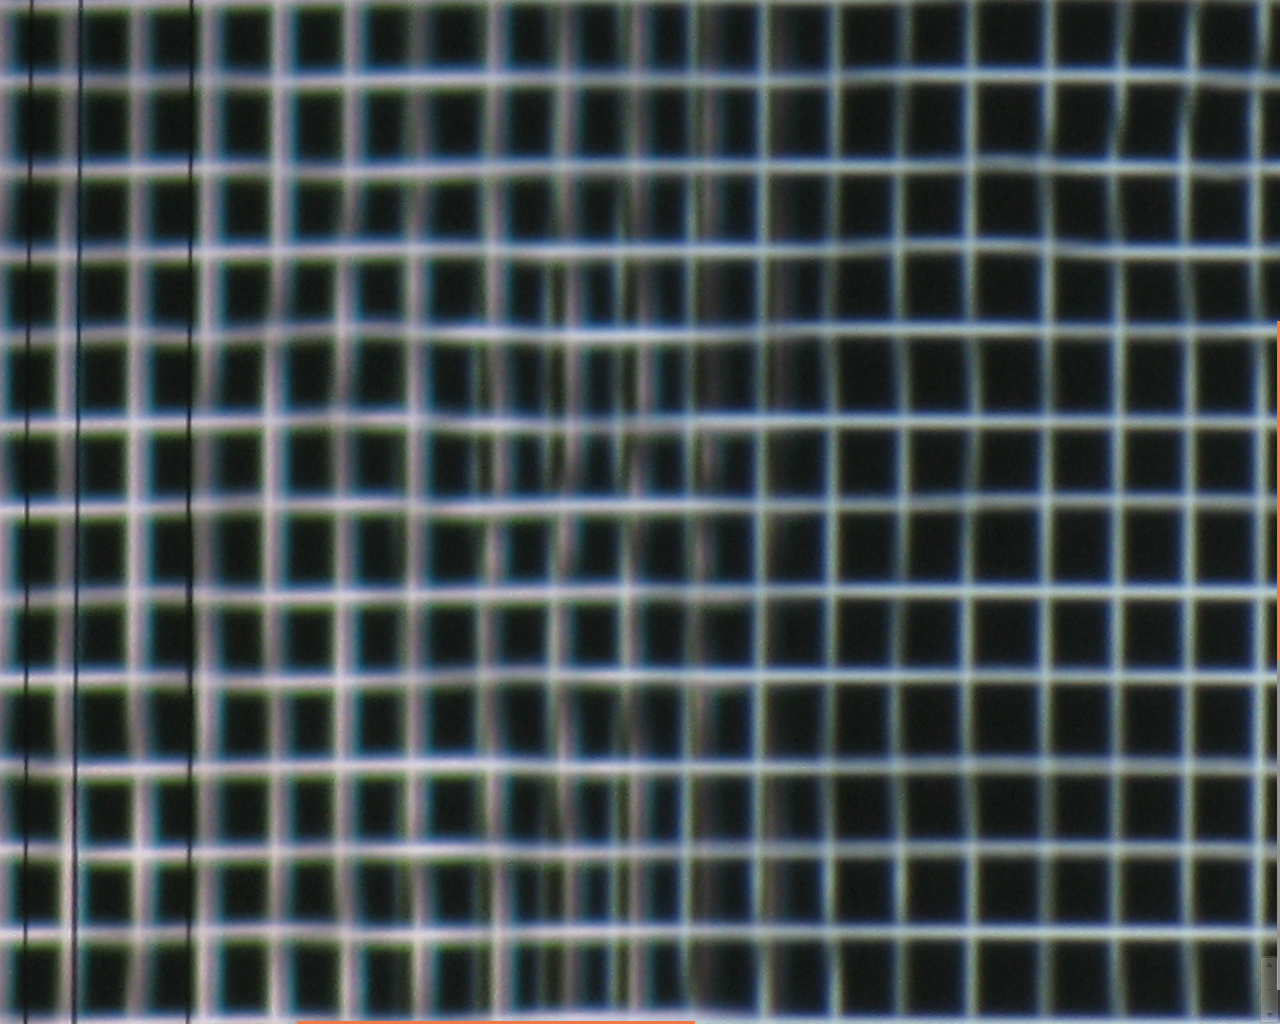
\includegraphics[width=6cm,height=4cm]{figures/misalign_1.png}
\caption{Magnified view of observed \textit{maximum} inter-projector misalignment}
\label{misalign}
\end{figure}


\section{Conclusion}
We have described an enhanced multiprojector geometric alignment utilizing \textit{Cross ratio} invariance based projection region recovery. Brown's method puts constraint and limitation in which atleast outer features of neighboring projector must overlap in order to get geometrically continuous image on the screen. This actually limits their claimed merit of casual alignment of projector. Further, there was no provision for using projection region beyond outermost features. Cross ratio approach allows for recovery of artificial feature points at the endpoints of a projection region due to which full projection region can be utilized and there is no constraint on projector positioning. Further, as shown in figures \ref{non_cross_rat} and \ref{cross_rat} using full projection region of each projector increases the area of overlap between neighboring projectors resulting in more uniform edge blending.


\section*{Acknowledgment}
Authors would like to thank Computer Graphics and Visualization section, Computer Division, BARC, Mumbai for providing valuable time, suggestions and infrastructure for this work.

\begin{thebibliography}{1}
\bibitem{1}
Ruddle, R.A.; Fateen, W.; Treanor, D.; Sondergeld, P.; Ouirke, P., "Leveraging wall-sized high-resolution displays for comparative genomics analyses of copy number variation," Biological Data Visualization (BioVis), 2013 IEEE Symposium on , vol., no., pp.89,96, 13-14 Oct. 2013

\bibitem{2} 
Brown, M.S.; Seales, W.B., ``A practical and flexible tiled display system,'' Computer Graphics and Applications, 2002. Proceedings. 10th Pacific Conference on , vol., no., pp.194,203, 2002


\bibitem{3}
Bose, S. K.; Sarode, D.M.; Venkata, P.P.K.; Shete, P.P.; Apte, A. G., "High End Scientific Visualization with Scalable Display System," Advances in Computer Engineering (ACE), 2010 International Conference on , vol., no., pp.316,318, 20-21 June 2010

\bibitem{4}
Nirnimesh; Harish, P.; Narayanan, P. J., "Garuda: A Scalable Tiled Display Wall Using Commodity PCs," Visualization and Computer Graphics, IEEE Transactions on , vol.13, no.5, pp.864,877, Sept.-Oct. 2007

\bibitem{5}
Weblink:\par
http://www.visbox.com/viswall-LCD.html


\bibitem{6}
Hereld, M.; Judson, I.R.; Stevens, R.L., "Introduction to building projection-based tiled display systems," Computer Graphics and Applications, IEEE , vol.20, no.4, pp.22,28, July-Aug. 2000

\bibitem{7}
Raskar, R.; Brown, M.S.; Ruigang Yang; Wei-Chao Chen; Welch, G.; Towles, H.; Scales, B.; Fuchs, H., "Multi-projector displays using camera-based registration," Visualization '99. Proceedings , vol., no., pp.161,522, 29-29 Oct. 1999

\bibitem{8} 
Brown, M.; Majumder, A.; Ruigang Yang, ``Camera-based calibration techniques for seamless multiprojector displays,'' Visualization and Computer Graphics, IEEE Transactions on , vol.11, no.2, pp.193,206, March-April 2005


\bibitem{9}
Dubrofsky, Elan. "Homography estimation." PhD diss., UNIVERSITY OF BRITISH COLUMBIA, 2009.

\bibitem{10}
Greg Humphreys, Mike Houston, Ren Ng, Randall Frank, Sean Ahern, Peter D. Kirchner, and James T. Klosowski. 2002. Chromium: a stream-processing framework for interactive rendering on clusters. ACM Trans. Graph. 21, 3 (July 2002), 693-702. 



\end{thebibliography}
\end{document}
